

O primeiro pacote trata de indentação e é bastante simples. Caso queira acessar e ler todas as quatro linhas de código do pacote \texttt{indentfirst}\index{indentfirst}, você pode acessá-lo em \url{http://mirrors.ctan.org/macros/latex/required/tools/indentfirst.pdf} \parencite{indentfirst}. Este pacote faz uma indentação obrigatória do primeiro parágrafo após o título de uma seção.

Já o pacote \texttt{setspace}\index{setspace} permite que se controle o espaçamento entre linhas de maneira bem simples, usando os comandos \texttt{\textbackslash singlespacing}\index{singlespacing}, \texttt{\textbackslash onehalfspacing}\index{onehalfspacing} e \texttt{\textbackslash doublespacing}\index{doublespacing}. Devido a sua simplicidade, esse pacote não possui manual. É importante dizer que existem outras maneiras de definir o espaçamento entre linhas em um documento, como utilizando os comandos \texttt{\textbackslash baselineskip}\index{baselineskip} ou \texttt{\textbackslash linespread},\index{linespread} como pode ser visto nas páginas do \gls{overleaf}\index{Overleaf} em \url{https://www.overleaf.com/learn/latex/paragraph_formatting}.

\section{Ajustes Finos}
O pacote \texttt{microtype}\index{microtype} provê uma interface para extensões micro-tipográficas introduzidas pelo \hologo{pdfLaTeX}\index{\hologo{pdfLaTeX}}, como protrusão de caracteres\footnote{A protrusão de caracteres move caracteres (geralmente pontuação), parcialmente ou integralmente, para a margem, de modo a criar uma aparência visualmente mais suave.}, expansão de fontes e ajustes finos entre palavras. Esse é um pacote que também pode ser usado com bons resultados na produção de artigos, e seu manual está disponível em \url{http://mirrors.ctan.org/macros/latex/contrib/microtype/microtype.pdf} \parencite{microtype}\index{microtype}.

\section{Cores}

O uso de cores para sinalizar mudanças ou chamar a atenção do leitor é algo comum e efetivo. Neste modelo, usamos o pacote \texttt{xcolor}\index{xcolor}. Assim, usando o comando: 

\adjustbox{fbox, center}{\texttt{\textbackslash textcolor\{red\}\{Texto com cor alterada.\}}}

\noindent pode-se produzir a seguinte saída:

\adjustbox{fbox, center}{\textcolor{red}{Texto com cor alterada.}}

Para maiores detalhes sobre o pacote \texttt{xcolor}, como opções do pacote, modelos de cores suportados e nomes de cores pré-definidos, consulte o manual no endereço \url{http://mirrors.ctan.org/macros/latex/contrib/xcolor/xcolor.pdf} \parencite{xcolor}.

\section{Contadores}

Neste modelo, escolhemos numerar os objetos float (figuras, tabelas e algoritmos) por capítulo. No modelo ABN\TeX{}\index{ABN\TeX{}}, essas contagens eram feitas de modo global. No \gls{scrbook}\index{scrbook}, a opção de contagem por capítulo é a padrão. 

Caso estivesse usando o modelo ABN\TeX{}\index{ABN\TeX{}}, você deveria usar os comandos abaixo para configurar a contagem por capítulos:

\begin{itemize}
	\item 
	\textbackslash \texttt{counterwithin\{figure\}\{chapter\}} - Define numeração de figuras por capítulo;
    \item \textbackslash \texttt{counterwithin\{table\}\{chapter\}} - Define numeração de tabelas por capítulo;
    \item \textbackslash \texttt{counterwithin\{algocf\}\{chapter\}} - Define numeração de algoritmos por capítulo;
\end{itemize}

Porém, se o seu processador \LaTeX{} for anterior a Abril de 2018, para usar o comando \texttt{counterwithin}\index{counterwithin} você deve usar o pacote \texttt{chngctr}\index{chngctr}.

Você pode resetar e acessar valores de contadores e até criar novos contadores. Um bom guia inicial de como usar contadores pode ser visto no \gls{overleaf}\index{Overleaf} (\url{https://www.overleaf.com/learn/latex/Counters}). Entretanto, sugiro que tenha cuidado ao manipular contadores, de modo a evitar problemas de numerações erradas em referências.

\section{Listas}

Quando utilizamos os ambientes \texttt{itemize\index{itemize}, enumerate\index{enumerate}} e  \texttt{description}\index{description} do \LaTeX{}, nós fazemos uso dos padrões de numeração definidos pelo \LaTeX{}. Caso desejemos alterar cesses padrões, podemos usar o pacote \texttt{enumitem}\index{enumitem}, que permite que o usuário controle o layout dos três ambientes citados acima, incluindo espaçamento, rótulos e numeração.

Você pode, por exemplo, remover o espaço vertical em uma lista usando a opção \texttt{nosep}\index{nosep}, como vemos abaixo no caso da definição de um ambiente \texttt{enumerate}: 

\adjustbox{fbox, center}{\textbackslash begin\{enumerate\}[nosep]}

Para maiores detalhes, consulte o manual do pacote, disponível em
\url{http://mirrors.ctan.org/macros/latex/contrib/enumitem/enumitem.pdf} \parencite{enumitem}.

Você pode ver em algum lugar referências a \LaTeXe{}. O \LaTeXe{} nada mais é do que a versão atual do \LaTeX{}. Uma nova versão, chamada de \LaTeX{}3, vem sendo desenvolvida há mais de uma década e deve ser lançada em alguns anos. Essas versões são referentes a linguagem, seus comandos e estrutura interna, e não às versões dos processadores \TeX{} e \LaTeX{}.

Este capítulo descreve a estrutura geral do modelo \LaTeX{} do \gls{ppgsc}, que foi feito usando a classe \texttt{scrbook} da família de pacotes \gls{koma}\index{\hologo{KOMAScript}} \parencite{koma}. As principais razões por trás desta escolha são uma maior flexibilidade em sua configuração e um menor número de conflitos com outros pacotes, quando comparado com as classes base \texttt{book} e \texttt{memoir}. 

Algumas explicações sobre os objetivos e formato deste documento são necessárias para que você compreenda como foi feito e possa utilizá-lo da melhor maneira. O principal objetivo deste documento é a homogeneização das dissertações e teses escritas no âmbito do \gls{ppgsc} da \gls{ufrn}, sendo que o \gls{ppgsc} é ligado diretamente ao \gls{ccet} e possui a grande maioria de seus professores lotados no \gls{dimap}. O segundo objetivo da elaboração do modelo e deste manual é o auxílio a ser dado aos alunos na escrita de suas qualificações, dissertações e teses.

Dados estes objetivos, decidi escrever este manual contendo informações sobre os pacotes, variáveis e parâmetros utilizados, no formato de uma dissertação, embora não seja o mais adequado para a escrita de um manual. Assim, você pode ter uma ideia melhor de como seu documento será organizado. Como consequência ou efeito colateral do uso de um modelo de dissertação para escrever esse manual, alguns nomes fantasia foram utilizados na sua escrita de modo a poupar terceiros do uso de seus nomes.

Espero que apreciem este documento e que o mesmo os auxiliem na escrita de seus trabalhos. Gostaria de salientar que tenho uma boa experiência com \LaTeX , mas estou bem longe de me considerar um \textit{expert} na matéria. Sugestões e correções são bem vindas.

Existem muitas referências de excelente qualidade sobre como elaborar documentos em \LaTeX . Listo a seguir algumas delas com breves descrições de seus conteúdos e objetivos. Os livros mais antigos ainda servem como textos base para os comandos do \LaTeX{}, embora o conteúdo sobre pacotes esteja desatualizado. No caso dos pacotes, o mais aconselhado é o uso dos manuais oficiais, guias rápidos e exemplos disponíveis na Internet.

\begin{itemize}
	\item \TeX{} StackExchange (\url{https://tex.stackexchange.com/}) - Extremamente útil, este sítio coleta dúvidas de usuários e respostas de especialistas em todo o mundo. Se você tem alguma dúvida sobre \TeX ou \LaTeX , ela provavelmente já foi perguntada e respondida lá.
	
	\item \gls{ctan} - Repositório de pacotes \LaTeX , também possui muitos manuais com vários exemplos de uso dos pacotes.
	
	\item \textit{\LaTeX{} (2nd Ed.): A Document Preparation System: User's Guide and Reference Manual} \parencite{Lamport1994}. Livro texto do criador do \LaTeX{}, Leslie Lamport, que descreve a linguagem \LaTeX{}, composta de comandos de alto nível, também chamados de macros, que simplificam o uso de \TeX{}.
	
	\item \textit{The \LaTeX{} Companion} \parencite{Mittelbach1999} - Ótima referência sobre \LaTeX{} e vários pacotes, embora esteja desatualizada em relação a novos pacotes.
	
	\item \textit{\LaTeX{} Graphics Companion, The (2nd Edition)} \parencite{Goosens2007} - Referência antiga, porém detalhada sobre como lidar com gráficos em documentos \LaTeX{}, comandos de desenho do PSTricks\index{PSTricks}, dentre outros. Como a referência anterior, esta serve como texto introdutório. 
	
	\item \textit{Typesetting Tables with \LaTeX{}} \parencite{Voss2011} - Esse livro se dedica exclusivamente a formatação de tabelas em \LaTeX{}.
	
	\item \textit{\LaTeX{} for Complete Novices} \parencite{Talbot2012} - Este livro introdutório é um bom guia para quem tem pouca experiência escrevendo documentos em \LaTeX{} e está disponível gratuitamente no endereço \url{https://www.dickimaw-books.com/latex/novices/novices-report.pdf} 
	
	\item \textit{\LaTeX{} Cookbook} \parencite{Kottwitz2015} - Livro recente, que inclui material sobre pacotes usados nesse modelo, como \gls{koma}\index{\hologo{KOMAScript}}, \gls{tikz}\index{Ti\textit{k}Z}, \texttt{pgfplots}\index{PGFPlots}, e BIB\LaTeX\index{biblatex}. Indicado para quem já tem um bom conhecimento sobre \LaTeX{}.
	
	\item \gls{overleaf} - Este sítio de escrita colaborativa de documentos em \LaTeX{} possui uma variada gama de artigos descrevendo o uso de vários comandos e pacotes, e é uma ótima opção para o compartilhamento de textos com seu(ua) orientador(a).
	
\end{itemize}

\section{Pacotes}

Ao longo deste documento, descreverei brevemente vários pacotes e algumas de suas funcionalidades e sintaxes. O objetivo deste manual é facilitar a escrita de documentos em \LaTeX{} no modelo \gls{ppgsc}, e o não detalhar os vários pacotes que foram sugeridos, testados e incluídos neste modelo. É importante frisar que provavelmente você não precisará utilizar a maioria dos pacotes citados aqui, e que basta comentar as linhas \texttt{\textbackslash usepackage\{pacote\}} do arquivo \texttt{./fixos/pacotes.tex}.

A grande maioria dos pacotes mencionados aqui estão disponíveis no \gls{ctan} e podem ser acessados em \url{https://ctan.org/}. Ao longo deste documento, incluirei links para os manuais oficiais dos pacotes, bem como para outras referências que proveêm conteúdo mais aprofundado sobre os mesmos.

\section{Codificação de Entrada e Fontes}

Vários pacotes que controlam a codificação de entrada e carregam fontes utilizadas no modelo são descritos a seguir.

\begin{itemize}
	\item \texttt{inputenc}\index{inputenc}
	
O pacote \texttt{inputenc} permite que o usuário especifique um padrão de codificação da entrada, i.e., dos caracteres. Existem dezenas de opções de codificação. Neste modelo, usamos o padrão \gls{utf}, definido no arquivo \texttt{Pacotes.tex}, e selecionado pelo comando: 

\adjustbox{fbox, center}{\texttt{\textbackslash{}usepackage[utf8]\{inputenc\}}}

O uso da codificação \gls{utf}\index{UTF} permite que seu documento use caracteres de várias linguagens, inclusive as que possuem caracteres não Latinos, além de vários símbolos usados em expressões matemáticas. Apesar do comando acima definir o conjunto de caracteres UTF como possíveis entradas, o mapeamento contido no arquivo \texttt{utf8.def} não contém mapeamentos de todos os possíveis caracteres \gls{utf}. Isso acontece devido ao imenso número de caracteres \gls{utf} que podem aparecer em um documento. Eu menciono isso porque os caracteres \gls{utf} não mapeados em utf8.def irão produzir uma mensagem de erro. Se isso acontecer, você deve incluir o mapeamento para este novo glifo\footnote{Glifo é a representação pictorial de um caractere.} no arquivo \texttt{utf8ienc.dtx} e carregá-lo no seu documento. Não acredito que você passará por essa experiência, a não ser que deseje incluir glifos de linguagens Asiáticas. 

O manual deste pacote pode ser acessado em 
\url{http://mirrors.ctan.org/macros/latex/base/inputenc.pdf} \parencite{inputenc}.

\item \texttt{fontenc}\index{fontenc}

O pacote \texttt{fontenc} permite que se selecione padrões de codificação de fontes usadas no documento. Neste modelo definimos as fontes como tendo codificação \texttt{T1}, que utiliza 8 bits, provendo espaço para 256 glifos. Isso permite que palavras com letras com acentos possam ser hifenizadas e que se possa copiar palavras acentuadas de outros documentos e os caracteres corretos sejam colados no seu documento. Além disso, alguns outros símbolos, como $>$, podem exibir um comportamento inesperado. O comando utilizado aqui é:

\adjustbox{fbox, center}{\texttt{\textbackslash usepackage[T1]\{fontenc\}}}

Esse pacote não possui um manual específico no \gls{ctan}\index{CTAN} pois faz parte do núcleo do \LaTeX{}.

\item \texttt{fontawesome}\index{fontawesome}

O pacote \texttt{fontawesome} fornece acesso a um grande número de ícones relacionados com a \textit{web}. Dependendo do tema de sua dissertação/tese, esses símbolos podem ser úteis para dar um toque mais profissional em alguns desenhos ou descrições.


\adjustbox{fbox, center}{\texttt{\textbackslash usepackage\{fontawesome\}}}

Abaixo estão alguns dos glifos definidos em \texttt{fontawesome}. O manual deste pacote pode ser acessado em 
\url{http://mirrors.ctan.org/fonts/fontawesome/doc/fontawesome.pdf} \parencite{fontawesome}. Um exemplo de seu uso neste documento pode ser visto na Tabela \ref{tab:fontawesome}.

\begin{table}[htb]
	\begin{center}
	\begin{tabular}{|c|c|c|c|c|c|c|c|c|c|}
		\hline
		\faBattery[0] & \faBattery[1] & \faBattery[2] & \faBattery[3] & \faBattery[4] & \faBarChart & \faBarcode & \faBluetooth & \faBeer & \faCalculator \\ \hline \faCalendar & \faClockO & \faClone & \faCloudDownload & \faCloudDownload & \faCodeFork &c\faCopy & \faCopyright & \faCreativeCommons & \faHotel \\ \hline
		\faFolder & \faFolderOpen & \faFolderO & \faFolderOpenO & \faGears & \faDesktop & \faLaptop & \faMobile & \faFile & \faFilePdfO \\ \hline 
		\faFilePhotoO & \faFilePowerpointO & \faFileSoundO & \faFileSoundO & \faFileTextO & \faFileVideoO & \faFileWordO & \faFileZipO & \faFilm & \faRebel \\ \hline
		\faAndroid & \faGoogle & \faAmazon & \faOpera & \faGithub & \faGitlab & \faFacebook & \faChrome & \faInstagram & \faInternetExplorer  \\ \hline 
		\faJoomla &	\faLinux & \faApple & \faSafari & \faSkype &  \faSnapchat & \faSpotify & \faTwitter & \faWikipediaW & \faWindows \\ \hline
	\end{tabular}
    \end{center}
    \caption{Exemplos de glifos do pacote \texttt{fontawesome}.}
    \label{tab:fontawesome}
\end{table}

\item \texttt{cmap}\index{cmap}

O pacote \texttt{cmap} provê tabelas de mapeamento de caracteres que permitem que arquivos gerados usando \hologo{pdfLaTeX} sejam buscáveis e seu conteúdo possa ser copiado na maioria dos visualizadores de arquivos \gls{pdf}.

\adjustbox{fbox, center}{\texttt{\textbackslash usepackage\{cmap\}}}

\item \texttt{lmodern}\index{lmodern}

O pacote \texttt{lmodern} provê a fonte Latin Modern, usada no modelo, e é carregado usando o comando abaixo.

\adjustbox{fbox, center}{\texttt{\textbackslash usepackage\{lmodern\}}}

\end{itemize}

\section{Estrutura de Arquivos}
Organizamos todos os arquivos do modelo em vários diretórios, de modo a compartimentalizar os arquivos de acordo com suas características e isolar os arquivos que não necessitam ser alterados por você.

Abaixo temos um exemplo da estrutura de arquivos utilizada para gerar um documento com 5 capítulos. Os nomes dos arquivos dos capítulos são de sua escolha e devem ser alterados nos comandos que os carregam, no arquivo principal, \texttt{DissertacaoPPgSC.tex}, cujo nome também pode ser mudado por você.

A estrutura de arquivos do modelo pode ser vista na Figura \ref{fig:est-arq} e mostra os arquivos \texttt{.tex}\index{.tex} que se localizam na pasta \texttt{capitulos}, que contêm o código fonte \LaTeX dos capítulos da dissertação/tese. Já o diretório \texttt{editaveis}, como o nome sugere, agrupa os arquivos \texttt{.tex} que devem ser alterados por você para que o documento tenha as informações específicas de seu trabalho e sua defesa. Já os arquivos do diretório \texttt{fixos} mostra os arquivos \texttt{.tex} que não devem ser alterados por você, exceto em caso de extrema necessidade. Finalmente, o diretório  \texttt{imagens} agrupa os diretórios que contêm os arquivos de imagens, organizados por capítulos, e com um diretório específico para os logotipos da \gls{ufrn} e \gls{ppgsc}. Essa figura foi gerada usando símbolos da fonte \texttt{fontawesome}, vista anteriormente, e o pacote Ti\textit{k}Z\index{Ti\textit{k}Z} (Seção \ref{sec:tikz}).

\begin{figure}
	\begin{center}
\begin{tikzpicture}[%
	grow via three points={one child at (0.5,-0.7) and
		two children at (0.5,-0.7) and (0.5,-1.4)},
	edge from parent path={(\tikzparentnode.south) |- (\tikzchildnode.west)}]
	\tikzstyle{every node}=[draw=black,thick,anchor=west]
	\node[font=\footnotesize] {\faFolderO \space diretório base}
	child { node[font=\footnotesize] {\faFileText \space DissertacaoPPgSC.tex}}
		child { node[font=\footnotesize] {\faFolder \space capitulos}
%			child { node[font=\footnotesize] {\faFileText \space Capitulo1.tex}}
%			child { node[font=\footnotesize] {\faFileText \space Capitulo2.tex}}
%			child { node[font=\footnotesize] {\faFileText \space Capitulo3.tex}}
%			child { node[font=\footnotesize] {\faFileText \space Capitulo4.tex}}
%			child { node[font=\footnotesize] {\faFileText \space Capitulo5.tex}}
		}
%		child [missing] {}				
%		child [missing] {}				
%		child [missing] {}				
%		child [missing] {}				
%		child [missing] {}	
		child { node[font=\footnotesize] {\faFolderO \space editaveis}
			child { node[font=\footnotesize] {\faFileText \space Abstract.tex}}
			child { node[font=\footnotesize] {\faFileText \space Acronimos.tex}}
			child { node[font=\footnotesize] {\faFileText \space Agradecimentos.tex}}
			child { node[font=\footnotesize] {\faFileText \space Dedicatoria.tex}}
			child { node[font=\footnotesize] {\faFileText \space Epigrafe.tex}}
			child { node[font=\footnotesize] {\faFileText \space FolhaDeAprovacao.tex}}
			child { node[font=\footnotesize] {\faFileText \space Informacoes.tex}}
			child { node[font=\footnotesize] {\faFileText \space Referencias.bib}}
			child { node[font=\footnotesize] {\faFileText \space Resumo.tex}}
			child { node[font=\footnotesize] {\faFileText \space Variaveis.tex}}
		}
		child [missing] {}				
		child [missing] {}				
		child [missing] {}				
		child [missing] {}				
		child [missing] {}	
		child [missing] {}				
		child [missing] {}				
		child [missing] {}				
		child [missing] {}				
		child [missing] {}	
		child { node {\faFolderO \space fixos}
			child { node[font=\footnotesize] {\faFileText \space Informacoes.tex}}
			child { node[font=\footnotesize] {\faFileText \space NovosComandos.tex}}
			child { node[font=\footnotesize] {\faFileText \space Pacotes.tex}}
		}		
		child [missing] {}				
		child [missing] {}				
		child [missing] {}	
		child { node[font=\footnotesize] {\faFolderO \space imagens}
			child { node[font=\footnotesize] {\faFolderO \space logos}
				child { node[font=\footnotesize] {\faFileImageO \space Brasao-UFRN.jpg}}
				child { node[font=\footnotesize] {\faFileImageO \space logo-ppgsc.png}}
			}
			child [missing] {}				
			child [missing] {}	
			child { node[font=\footnotesize] {\faFolder \space capitulo1}}
			child { node[font=\footnotesize] {\faFolder \space capitulo2}}
			child { node[font=\footnotesize] {\faFolder \space capitulo3}}
			child { node[font=\footnotesize] {\faFolder \space capitulo4}}
			child { node[font=\footnotesize] {\faFolder \space capitulo5}}
		};
\end{tikzpicture}
\end{center}
\caption{Estrutura de arquivos do modelo PPgSC. Essa figura foi gerada usando Ti\textit{k}Z (ver Capítulo \ref{cap:desenhos}) e os símbolos da fonte \texttt{fontawesome}.}
\label{fig:est-arq}
\end{figure}

\section{Linguagens}

O pacote \texttt{babel}\index{babel} gerencia regras tipográficas para uma grande game de linguagens. Usando este pacote, um documento pode selecionar uma ou mais linguagens para serem usadas, e alternar entre as linguagens quando necessário. 

O comando utilizado neste modelo usa a opção \texttt{brazil}\index{brazil} (como pode ser visto abaixo), que define os nomes dos elementos como Conteúdo, Lista de Figuras, etc.

\adjustbox{fbox, center}{\textbackslash\texttt{usepackage[brazil]\{babel\}}}

Na realidade, qualquer das opções \texttt{brazil}\index{brazil}, \texttt{brazilian}\index{brazilian}, \texttt{portuges}\index{portuges} ou \texttt{portuguese}\index{portuguese} são aceitas e têm o mesmo efeito. O manual do \texttt{babel}\index{babel} pode ser acessado em \url{http://mirrors.ctan.org/macros/latex/required/babel/base/babel.pdf} \parencite{babel}.

Entretanto, para que o babel funcione com Português é preciso que você também tenha o pacote \texttt{babel-portuges}\index{babel-portuges} instalado. Este pacote é o que realmente define as macros específicas e é carregado automaticamente pelo \texttt{babel}\index{babel}. Garanta também que o pacote \texttt{hyphen-portuguese}\index{hyphen-portuguese} esteja instalado. O manual do \texttt{babel-portuges} pode ser acessado em \url{http://mirrors.ctan.org/macros/latex/contrib/babel-contrib/portuges/portuges.pdf} \parencite{babel-portuges}.

\section{Variáveis}
O modelo define algumas variáveis de modo a facilitar a geração das páginas iniciais do documento, e que são definidas no arquivo \texttt{./fixos/variaveis.tex}. Os nomes, tipos e significados das variáveis são:

\begin{itemize}
	\item \texttt{PPgSC-Proposta}\index{PPgSC-Tese} - Variável do tipo booleano que indica se o documento é um documento de exame preliminar (qualificação de mestrado ou proposta de doutorado) ou se é um documento de exame final (dissertação ou tese); Valor default: \texttt{false}.
	\item \texttt{PPgSC-Tese}\index{PPgSC-Tese} - Variável do tipo booleano que indica se o documento é uma tese de doutorado; Valor default: \texttt{false}.
	\item \texttt{PPgSC-Ingles}\index{PPgSC-Ingles} - Variável do tipo booleano que indica se a linguagem usada na escrita do documento é o Inglês; Valor default: \texttt{false}.
	\item \texttt{CO-orientador}\index{CO-orientador} - Variável do tipo booleano que indica se o aluno(a) possui Coorientador(a); Valor default: \texttt{false}.
	\item \texttt{signSkip}\index{signSkip} - Variável numérica que indica o espaço usado no espaçamento vertical de uma linha de assinatura; Valor default: \si{1.3cm}.
	\item \texttt{signWidth}\index{signWidth} - Variável numérica que indica o comprimento de uma linha de assinatura; Valor default: \si{10cm}.
	\item \texttt{signThickness}\index{signThickness} - Variável numérica que indica a espessura de uma linha de assinatura;  Valor default: \si{0,4pt}.
\end{itemize}

É importante lembrar que os comandos, variáveis e macros em \LaTeX{} são \textit{case sensitive}, i.e., se você não usar letras minúsculas e maiúsculas nos lugares corretos, o \LaTeX{} não vai reconhecer os comandos e variáveis.

\section{Novos Comandos}
Alguns novos comandos foram criados para facilitar a diagramação, como a capa do documento, a folha de assinaturas, e o \textit{Abstract} e o Resumo, que não fazem parte da classe \gls{scrbook} da \gls{koma}\index{\hologo{KOMAScript}}.

O arquivo \texttt{./fixos/informacoes.tex} contém informações imutáveis sobre o programa e a instituição, enquanto que o arquivo  \texttt{./editaveis/informacoes.tex} contém informações específicas do trabalho, como autor, data, orientador, coorientador (se for o caso). Essas informações são utilizadas para gerar os elementos abaixo.

\begin{itemize}
	\item Capa - Página gerada automaticamente. Utiliza imagens dos logotipos da \gls{ufrn} e do \gls{ppgsc} e informações do arquivo \texttt{./editaveis/informacoes.tex}.
	\item Folha de rosto - Página gerada automaticamente. Utiliza  informações do arquivo \texttt{./editaveis/informacoes.tex}.
	\item Folha de assinaturas - Página que precisa ser ajustada manualmente, incluindo os nomes dos membros da banca que não são o orientador e coorientador no arquivo \texttt{./editaveis/FolhaDeAprovacao.tex}. 
	\item Abstract - Novo \textit{environment}\index{environment} (ambiente) definido no modelo devido a sua ausência no \gls{koma}. Está definido no arquivo \texttt{./fixos/NovosComandos.tex}.
	\item Resumo - Novo \textit{environment} (ambiente) definido no modelo devido a sua ausência no \gls{koma}. Está definido no arquivo \texttt{./fixos/NovosComandos.tex}.  
\end{itemize}

\section{Arquivos Auxiliares}

Um dos problemas existentes no \TeX{} que não foi resolvido na implementação do $\epsilon$-\TeX{} (\LaTeXe{}) foi o suporte a somente 18 manipuladores de arquivos para escrita (\textit{write handles}). Esse número pode parecer grande, mas muitos desses manipuladores são reservados, como o manipulador 0 para o arquivo \texttt{.log}\index{.log}. O \TeX{} usa o manipulador 1 para o arquivo \texttt{.aux}\index{.aux}, o 2 para o \texttt{partaux}\index{partaux}, e um manipulador para cada lista, como as geradas pelos comandos \texttt{\textbackslash{}tableofcontents}\index{tableofcontents},
\texttt{\textbackslash{}listoffigures}\index{listoffigures} e \texttt{\textbackslash{}listoftables}\index{listoftables}. Além disso, o \LaTeX{} usa manipuladores para pacotes como \texttt{\textbackslash{}makeindex}\index{makeindex}, \texttt{hyperref}\index{hyperref}, \texttt{minted}\index{minted}, Ti\textit{k}Z\index{Ti\textit{k}Z} e \texttt{glossaries}\index{glossaries}, que usa mais de um manipulador.

O problema aparece quando seu documento usa muitos desses pacotes que utilizam arquivos para armazenar informações que são utilizadas em passos extra do processador \LaTeX{} para formatar corretamente seu documento. Eventualmente, você pode receber a mensagem abaixo durante o processamento de seu documento. 

\adjustbox{fbox, center}{\texttt{ \texttt{!No room for a new \textbackslash{}write}}}

Por algum tempo, a solução mais simples adotada era a da utilização de \hologo{LuaLaTeX}\index{\hologo{LuaLaTeX}} ao invés de \hologo{pdfLaTeX}\index{\hologo{pdfLaTeX}} ou \hologo{XeLaTeX}\index{\hologo{XeLaTeX}}, eliminando esta restrição e limitando o número de manipuladores de arquivos abertos de acordo com o sistema operacional. O pacote \texttt{scrwfile}\index{scrwfile}, do \gls{koma}\index{\hologo{KOMAScript}}, altera o \textit{kernel}\index{kernel} do \LaTeX{}, permitindo que \hologo{pdfLaTeX} e \hologo{XeLaTeX} também possam utilizar mais do que 18 manipuladores de arquivos. Para mais detalhes, leia o Capítulo 14 de \parencite{koma}.

\section{Como Usar Este Modelo}

Para começar a utilizar este modelo de dissertações/teses, copie toda a estrutura de arquivos e comece a editar os arquivos que contêm informações sobre seu documento. Comece pelos arquivos do diretório \texttt{editaveis}, que podem ser vistos na Figura \ref{fig:est-arq}. Caso não deseje utilizar um ou mais elementos localizados nesse diretório, como \textbf{Dedicatória} ou \textbf{Agradecimentos}, comente sua inclusão no arquivo principal, o DissertacaoPPgSC.tex. 

O nome do arquivo principal pode ser alterado por você, bem como os nomes dos arquivos de referências bibliográficas e dos capítulos. Apenas se certifique que alterou seus nomes ao carregá-los no arquivo principal. A estrutura de organização das imagens também é sugerida, e pode ser alterada caso deseje. Sugiro que incluam novos pacotes no arquivo principal, caso necessitem, embora, em alguns casos, os autores indiquem a necessidade de precedência no carregamento de diferentes pacotes. Nesse caso, é mais prudente seguir as indicações dos autores dos pacotes que desejam usar.

Finalmente, não se esqueça de configurar sua \gls{ide} para que execute a sequência correta de comandos. Por exemplo, caso esteja usando BIB\LaTeX{} com \hologo{biber}, certifique-se que sua \gls{ide} chama o \hologo{biber} e não o \BibTeX{} (Capítulo \ref{cap:refs}). Em alguns casos, também é necessário incluir o flag \texttt{-shell-escape} na execução do \hologo{pdfLaTeX}, como no caso do pacote \texttt{minted} (Seção \ref{sec:codigo}).


% Capítulo 3
\chapter{Objetos Float - Figuras, Tabelas, Algoritmos e Código Fonte}\label{cap:float}

Neste capítulo, irei falar sobre objetos do tipo \texttt{float}, que recebem este nome porque ``flutuam'' no documento, e têm seus lugares finais influenciados por sugestões dadas pelos autores, mas que o \LaTeX{} tem a decisão final sobre onde os colocar. Os principais objetos \texttt{float}\index{float} são as figuras, tabelas, algoritmos e listagens de códigos. 

As seções a seguir contêm exemplos do uso desses quatro tipos de objetos \texttt{float}, bem como de alguns pacotes auxiliares que foram incorporados a este modelo de dissertação/tese.

O pacote \texttt{pdflscape}\index{pdflscape} adiciona o suporte \gls{pdf}\index{PDF} ao ambiente \textit{landscape}\index{landscape} (orientação paisagem) do pacote \texttt{lscape}\index{lscape}. Páginas marcadas com o atributo que indica essa orientação serão rotacionadas e mostradas em modo paisagem pelos visualizadores de arquivos \gls{pdf}. O manual desse pacote pode ser acessado em \url{http://mirrors.ctan.org/macros/latex/contrib/pdflscape/pdflscape.pdf} \parencite{pdflscape}.

O pacote \texttt{float}\index{float} melhora a interface para a definição de objetos \texttt{float}, introduzindo os objetos \textit{boxed float}\index{boxed float}, \textit{ruled float}\index{ruled float} e \textit{plaintop float}\index{plaintop float}. O primeiro tipo de objeto cria floats com um retângulo ao redor dos objetos, enquanto que os dois últimos tipos são mais usados para mostrar códigos. Entretanto, o pacote \texttt{minted}\index{minted}, mostrado na Seção \ref{sec:codigo} provê uma visualização muito mais elegante, de modo que sugiro que use o \texttt{minted} para diagramar seus códigos em \LaTeX{}.

O pacote \texttt{float} ainda define a opção \texttt{H} para colocação de \textit{floats}, que força o \LaTeX{} a colocar um objeto \texttt{float} exatamente naquele lugar (deixando assim de ser um objeto \texttt{float}), mesmo que isso implique em deixar uma parte da página anterior em branco, sem texto. Use essa opção com parcimônia, pois ela pode quebrar o seu texto e gerar uma diagramação esquisita. O manual do pacote \texttt{float}\index{float} pode ser acessado em \url{http://mirrors.ctan.org/macros/latex/contrib/float/float.pdf} \parencite{float}.

O pacote \texttt{adjustbox}\index{adjustbox} pode ser usado para ajustar conteúdo dentro de uma caixa ``virtual'', alterando sua escala, orientação e cortar parte do conteúdo. Esse pacote pode ser aplicado a qualquer objeto \texttt{float} ou até a texto. Os textos destacados dentro de caixas e centralizados que aparecem nos Capítulos \ref{cap:modelo}, \ref{cap:diagramacao}  e outros ainda não vistos, foram produzidos usando o pacote \texttt{adjustbox}. Você também pode usar o \texttt{adjustbox} para diminuir o tamanho de uma tabela, por exemplo, quando ela passa um pouco da largura máxima da área reservada para o texto, e uma diminuição da fonte usada gera letras muito pequenas, difíceis de se ver. Nesse caso, um pequeno ajuste do tamanho da tabela pode ser a melhor opção. Você deve usar essa opção com cuidado, pois uma mudança muito grande pode afetar a qualidade da saída.

\section{Figuras}

Como recomendo o uso do processador \hologo{pdfLaTeX}\index{\hologo{pdfLaTeX}}, devo informar que o \hologo{pdfLaTeX} permite carregar imagens nos formatos \gls{pdf}\index{PDF}, \gls{png}\index{PNG} e \gls{jpg}\index{JPG}. Algumas ferramentas, como LyX, fazem a conversão \textit{on-the-fly}, facilitando a tarefa do usuário mas adicionando tempo ao processamento do texto. Eu sugiro que você converta suas imagens para um desses formatos antes de carregá-las, economizando tempo de conversão durante a compilação do código \LaTeX{}.

O pacote \texttt{graphicx}\index{graphicx} se baseia no pacote \texttt{graphics}\index{graphics} para prover uma interface para argumentos opcionais para o comando \texttt{\textbackslash{}includegraphics}\index{includegraphics}. O pacote \texttt{graphicx} faz parte do grupo de pacotes \texttt{latex-graphics}\index{latex-graphics}, que é uma das coleções obrigatórias\footnote{As coleções obrigatórias de \LaTeX{} implicam que toda distribuição \LaTeX{} deve possuí-las.} de \LaTeX{}.

Na Figura \ref{fig:phdcomics}  vemos um exemplo do uso do comando \texttt{\textbackslash{}includegraphics} para a inclusão de uma imagem no objeto \texttt{float figure}. Os comandos utilizados para gerar essa figura podem ser vistos no Código \ref{cod:includegraphics}.

\begin{figure}[ht]
	\centering
	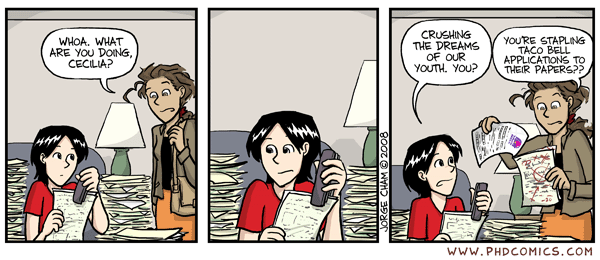
\includegraphics[width=14cm]{./imagens/capitulo3/phd020808s}
	\caption{Tirinha cômica extraída da página \url{phdcomics.com}.}
	\label{fig:phdcomics}
\end{figure}

\begin{listing}[ht]
	\begin{minted}[linenos=true, baselinestretch=1, autogobble, bgcolor=Cornsilk1]{tex}
		\begin{figure}[ht]
		  \centering
		  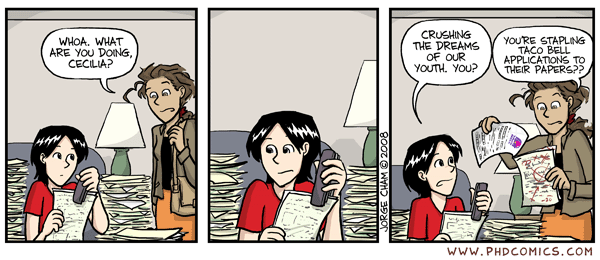
\includegraphics[width=12cm]{./imagens/capitulo3/phd020808s}
		  \caption{Tirinha cômica extraída da página \url{phdcomics.com}.}
		  \label{fig:phdcomics}
		\end{figure}
	\end{minted}
\caption{Exemplo de imagem carregada usando o comando \texttt{\textbackslash{}includegraphics}.}
\label{cod:includegraphics}
\end{listing}

O manual disponível em  \url{http://mirrors.ctan.org/macros/latex/required/graphics/grfguide.pdf} \parencite{graphicsguide} se refere à coleção \texttt{latex-graphics}\index{latex-graphics} e descreve os pacotes \texttt{color}\index{color}, \texttt{graphics}\index{graphics} e \texttt{graphicx}\index{graphicx} enquanto que o manual acessível em \url{http://mirrors.ctan.org/macros/latex/required/graphics/graphics.pdf} \parencite{graphics} descreve o pacote \texttt{graphics}. Sugiro a leitura do primeiro manual, principalmente das opções descritas em sua Seção 4.4, que tratam da formatação das imagens carregadas pelo comando \texttt{\textbackslash{}includegraphics}\index{includegraphics}.

\subsection{Sub-figuras}

O pacote \texttt{subfig}\index{subfig} provê suporte para a manipulação e referenciamento de subfiguras\index{subfiguras} e subtabelas\index{subtabelas}, permitindo que elas possam ser referenciadas e/ou descritas separadamente ou até mesmo listadas separadamente na Lista de Figuras. Um exemplo simples de figura composta por subfiguras e que foi contruída usando o pacote \texttt{subfig} pode ser vista na Figura \ref{fig:subfig}. Os comandos necessários para gerar esta figura podem ser vistos no Código \ref{cod:subfig}.

\begin{figure}[ht]
    \centering
    \subfloat[]{
        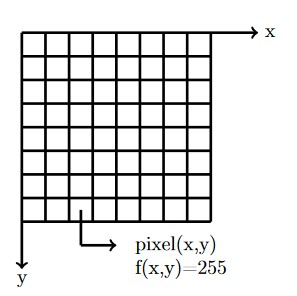
\includegraphics[height=5cm]{imagens/capitulo2/imagemCinza.jpg}}
    \subfloat[]{
        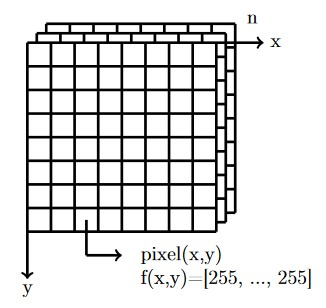
\includegraphics[height=5cm]{imagens/capitulo2/imagemColorida.jpg}}
    \caption{Exemplo de subfiguras usando o pacote \texttt{subfig}. Representação de uma imagem digital. (a) Imagem em escala de cinza. (b) Imagem colorida. Imagem extraída de \parencite{Barbosa2020}.}
    \label{fig:subfig}
\end{figure}

\begin{listing}[ht]
	\begin{minted}[linenos=true, baselinestretch=1, autogobble, bgcolor=Cornsilk1]{tex}
		\begin{figure}[ht]
		  \centering
		  \subfloat[]{
		    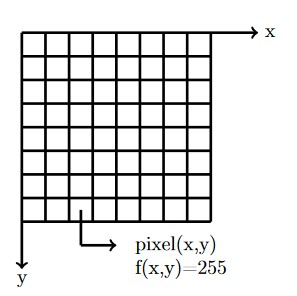
\includegraphics[height=5cm]{imagens/capitulo2/imagemCinza.jpg}}
		  \subfloat[]{
		    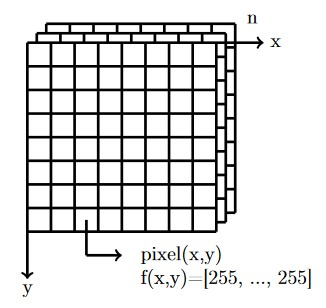
\includegraphics[height=5cm]{imagens/capitulo2/imagemColorida.jpg}}
		  \caption{Exemplo de subfiguras usando o pacote \texttt{subfig}. 
		  Representação de uma imagem digital. (a) Imagem em escala de cinza. 
		  (b) Imagem colorida. Imagem extraída de \parencite{Barbosa2020}.}
		  \label{fig:subfig}
		\end{figure}
	\end{minted}
	\caption{Código usado para organizar subfiguras usando o pacote \texttt{subfig}.}
	\label{cod:subfig}
\end{listing}

Como alternativa, você pode usar o ambiente \texttt{tabular}\index{tabular} para organizar as subfiguras e seus rótulos. A Figura \ref{fig:subfigtabular} foi criada usando este outro modo de organizar subfiguras. O Código \ref{cod:subfigtabular} mostra os comandos usados para gerá-la.

\begin{figure}[H]
	\begin{center}
		\begin{tabular}{cc}
			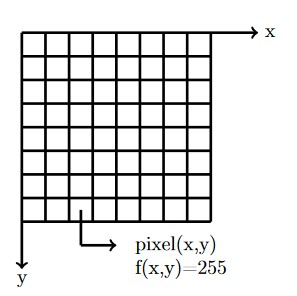
\includegraphics[height=5cm]{imagens/capitulo2/imagemCinza.jpg} & 
			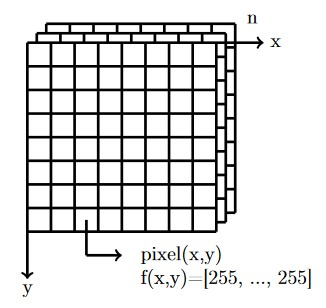
\includegraphics[height=5cm]{imagens/capitulo2/imagemColorida.jpg} \\
			(a) & (b) 
		\end{tabular}
	\end{center}
	\caption{Exemplo de subfiguras\index{subfiguras} usando o ambiente \texttt{tabular}. Representação de uma imagem digital. (a) Imagem em escala de cinza. (b) Imagem colorida. Imagem extraída de \parencite{Barbosa2020}.}
	\label{fig:subfigtabular}
\end{figure}

\begin{listing}[ht]
	\begin{minted}[linenos=true, baselinestretch=1, autogobble, bgcolor=Cornsilk1]{tex}
		\begin{figure}[ht]
		  \begin{center}
		    \begin{tabular}{cc}
		      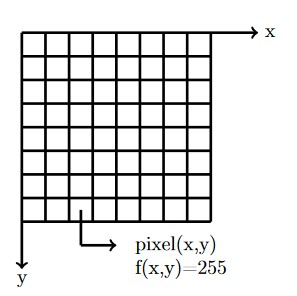
\includegraphics[height=5cm]{imagens/capitulo2/imagemCinza.jpg} & 
		      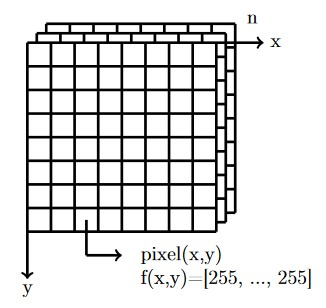
\includegraphics[height=5cm]{imagens/capitulo2/imagemColorida.jpg} 
		      \\
		      (a) & (b) 
		    \end{tabular}
		  \end{center}
		  \caption{Exemplo de subfiguras usando o ambiente \texttt{tabular}. 
		  Representação de uma imagem digital. (a) Imagem em escala de cinza. 
		  (b) Imagem colorida. Imagem extraída de \parencite{Barbosa2020}.}
		  \label{fig:subfigtabular}
		\end{figure}
	\end{minted}
	\caption{Código usado para organizar subfiguras usando o ambiente \texttt{tabular}.}
	\label{cod:subfigtabular}
\end{listing}

Você pode comparar visualmente os resultados das duas opções descritas acima observando as \Cref{fig:subfig,fig:subfigtabular}. Lembre-se que no caso do pacote \texttt{subfig}\index{subfig}, você pode referenciar e listar as subfiguras separadamente. Para maiores detalhes sobre o pacote \texttt{subfig}, consulte seu manual, que está disponível em \url{http://mirrors.ctan.org/macros/latex/contrib/subfig/subfig.pdf} \parencite{subfig}.

\section{Tabelas}

Tabelas são um outro tipo de objeto \texttt{float}\index{float} presente no \LaTeX{}. Existem páginas, capítulos de livros e até livros completos dedicados a criação de tabelas  em \LaTeX{}. Geralmente, se utiliza um ambiente tabular dentro de um objeto \texttt{float} do tipo \texttt{table}\index{table}. Esse ambiente tabular é responsável por informar quantas colunas uma tabela terá, e por sua tabulação, organizando os dados usando delimitadores pré-definidos.

\begin{table}[H]
	\centering
	\resizebox{\textwidth}{!}{%
		\begin{tabular}{|l|l|l|l|l|l|}
			\hline
			Tecido & Distância e Tamanho & Acurácia & Especificidade  & Sensibilidade & Coeficiente de Dice \\ \hline
			\multirow{2}{*}{Granulação} & $9 \times 9$\_E & $0,9252 \pm 0,0796$ & \textbf{$0,8961 \pm 0,1520$} & $0,8478 \pm 0,1942$ & $0,8796 \pm 0,1699$ \\ \cline{2-6}
			& $11 \times 11$\_E\_CSR & \textbf{$0,9292 \pm 0,0755$} & $0,8828 \pm 0,1673$ & \textbf{$0,8983 \pm 0,0914$} & \textbf{$0,9224 \pm 0,0650$} \\ \hline
			\multirow{2}{*}{Necrótico} & $9 \times 9$\_E & \textbf{$0,9595 \pm 0,0518$} & $0,9739 \pm 0,0436$ & $0,8758 \pm 0,8800$ & $0,8215 \pm 0,3155$ \\ \cline{2-6}
			& $11 \times 11$\_E\_CSR & $0,9591 \pm 0,0514$ & \textbf{$0,9741 \pm 0,0379$} & \textbf{$0,8963 \pm 0,0638$} & \textbf{$0,9037 \pm 0,1195$} \\  \hline
			\multirow{2}{*}{Esfacelo} & $9 \times 9$\_E & \textbf{$0,9346 \pm 0,0840$} & \textbf{$1,0000 \pm 0,0000$} & $0,8018 \pm 0,1489$ & \textbf{$0,8825 \pm 0,0983$} \\ \cline{2-6}
			& $11 \times 11$\_E\_CSR & $0,9336 \pm 0,0854$ & \textbf{$1,0000 \pm 0,0000$} & \textbf{$0,8111 \pm 0,1378$} & $0,8707 \pm 0,1089$ \\  \hline
			\multirow{2}{*}{Todos} & $9 \times 9$\_E & $0,9482 \pm 0,0457$ & $0,9784 \pm 0,0309$ & $0,8932 \pm 0,0771$ & $0,9234 \pm 0,0673$ \\ \cline{2-6}
			& $11 \times 11$\_E\_CSR & \textbf{$0,9491 \pm 0,0423$} & \textbf{$0,9788 \pm 0,0298$} & \textbf{$0,8952 \pm 0,0717$} & \textbf{$0,9247 \pm 0,0625$} \\ \hline
		\end{tabular}%
	}
	\caption{Resultados de uma tarefa de agrupamento. Adaptada de \parencite{Marques2018}.}
	\label{tab:resultadosVitor}
\end{table}

A Tabela \ref{tab:resultadosVitor} (adaptada de \parencite{Marques2018}) mostra resultados de uma tarefa de classificação. Neste exemplo, usei o pacote \texttt{multirow}\index{multirow} \parencite{multirow}, que permite criar multilinhas\index{multilinhas} e multicolunas\index{multicolunas}, centralizando o texto dentro dessas células compostas. O Código \ref{cod:tabresultadosVitor} mostra os comandos usados para gerar a Tabela \ref{tab:resultadosVitor}.

\begin{listing}[H]
	\begin{minted}[linenos=true, baselinestretch=1, autogobble, bgcolor=Cornsilk1]{tex}
	\begin{table}[H]
	  \centering
	  \resizebox{\textwidth}{!}{%
	  \begin{tabular}{|l|l|l|l|l|l|}
	    \hline
	    Tecido & Distância e Tamanho & Acurácia & Especificidade  
	    & Sensibilidade & Coeficiente de Dice \\ \hline
	    \multirow{2}{*}{Granulação} & $9 \times 9$\_E & $0,9252 
	    \pm 0,0796$ & \textbf{$0,8961 \pm 0,1520$} & $0,8478 \pm 0,1942$ 
	    & $0,8796 \pm 0,1699$ \\ \cline{2-6}
	    & $11 \times 11$\_\_CSR & \textbf{$0,9292 \pm 0,0755$} & 
	    $0,8828 \pm 0,1673$ & \textbf{$0,8983 \pm 0,0914$} & 
	    \textbf{$0,9224 \pm 0,0650$} \\ \hline
	    \multirow{2}{*}{Necrótico} & $9 \times 9$\_E & 
	    \textbf{$0,9595 \pm 0,0518$} & $0,9739 \pm 0,0436$ &
	    $0,8758 \pm 0,8800$ & $0,8215 \pm 0,3155$ \\ \cline{2-6}
	    & $11 \times 11$\_E\_CSR & $0,9591 \pm 0,0514$ & 
	    \textbf{$0,9741 \pm 0,0379$} & \textbf{$0,8963 \pm
	    0,0638$} & \textbf{$0,9037 \pm 0,1195$} \\ \hline
	    \multirow{2}{*}{Esfacelo} & $9 \times 9$\_E & 
	    \textbf{$0,9346 \pm 0,0840$} & \textbf{$1,0000 \pm
	    0,0000$} & $0,8018 \pm 0,1489$ & \textbf{$0,8825 \pm
	    0,0983$} \\ \cline{2-6}
	    & $11 \times 11$\_E\_CSR & $0,9336 \pm 0,0854$ & 
	    \textbf{$1,0000 \pm 0,0000$} & \textbf{$0,8111 \pm
	    0,1378$} & $0,8707 \pm 0,1089$ \\ \hline
	    \multirow{2}{*}{Todos} & $9 \times 9$\_E & $0,9482 
	    \pm 0,0457$ & $0,9784 \pm 0,0309$ & $0,8932 \pm 
	    0,0771$ & $0,9234 \pm 0,0673$ \\ \cline{2-6}
	    & $11 \times 11$\_E\_CSR & \textbf{$0,9491 \pm 0,0423$} 
	    & \textbf{$0,9788 \pm 0,0298$} & \textbf{$0,8952 \pm 0,0717$} & 
	    \textbf{$0,9247 \pm 0,0625$} \\ \hline
	  \end{tabular}%
	  }
	  \caption{Melhores resultados do agrupamento, adaptada de 
	  \parencite{Marques2018}.}
	  \label{tab:resultadosVitor}
	\end{table}
	\end{minted}
	\caption{Código usado para gerar a Tabela \ref{tab:resultadosVitor}.}
	\label{cod:tabresultadosVitor}
\end{listing}

Além do estilo padrão de tabelas do \LaTeX{}, que é bem permissivo, pode-se utilizar o pacote \texttt{booktabs}\index{booktabs} \parencite{booktabs}, que é conhecido pelo estilo de suas tabelas, similar a tabelas presentes em livros. Entretanto, o \texttt{booktabs} tem algumas restrições que foram impostas por escolhas de diagramação feitas pelos seus autores, como a impossibilidade de se usar linhas verticais separando colunas de uma tabela, a adição de um espaço acima e abaixo de linhas horizontais, a existência de linhas de diferentes espessuras e a impossibilidade do uso de linhas de separação duplas. Assim como as tabelas do estilo padrão do \LaTeX{}, as tabelas do \texttt{booktabs} podem ter suas linhas ou colunas coloridas usando os pacotes \texttt{xcolor}\index{xcolor} ou \texttt{colortbl}\index{colortbl}. O manual do pacote \texttt{booktabs} pode ser acessado em \url{http://mirrors.ctan.org/macros/latex/contrib/booktabs/booktabs.pdf} \parencite{booktabs}. 

Caso você tenha problemas no início para gerar suas tabelas, você pode utilizar algumas das páginas na Internet que permitem a criação de tabelas em \LaTeX{} de modo interativo, como o Tables Generator\index{Tables Generator} (\url{https://www.tablesgenerator.com/}) e o \LaTeX{} Tables\index{\LaTeX{} Tables} (\url{https://www.latex-tables.com/}). Algumas delas ainda permitem que se importem dados de arquivos de vários tipos, como \texttt{.csv}\index{.csv}, \texttt{.xls}\index{.xls} e \texttt{.ods}\index{.ods}.

Se você desejar criar tabelas muito elaboradas, podendo inclusive conter ilustrações, então eu sugiro que considere criá-las usando Ti\textit{k}Z\index{Ti\textit{k}Z}, que será abordado no Capítulo \ref{cap:desenhos}. Vários exemplos de tabelas criadas usando Ti\textit{k}Z estão disponíveis na Internet. 

\section{Algoritmos}

O pacote \texttt{algorithm2e}\index{algorithm2e} define um ambiente para escrever algoritmos em \LaTeXe, que são definidos como objetos \textit{float}\index{float} como figuras e tabelas. A apresentação dos algoritmos é bastante configurável.  As opções mostradas no Código \ref{cod:algorithm2e-setup} indicam que os algoritmos serão numerados por capítulo (\texttt{algochapter}\index{algochapter}), terão suas linhas numeradas (\texttt{linesnumbered}\index{linesnumbered}), exceto por comentários e entrada/saída, imprime linhas verticais delimitando blocos (\texttt{lined}\index{lined}), usa as palavras chaves em Português (portuguese) e escolhe o estilo \texttt{ruled}\index{ruled} como padrão para mostrar os algoritmos.

\begin{listing}[ht]
	\begin{minted}[linenos=true, autogobble, bgcolor=Cornsilk1]{tex}
	  \usepackage[algochapter, linesnumbered, lined, portuguese, ruled]
	  {algorithm2e}
	\end{minted}
	\caption{Exemplo de código \LaTeX{} usado para configuração do \texttt{algorithm2e}.}
	\label{cod:algorithm2e-setup}
\end{listing}

\begin{algorithm}[ht]
  \setstretch{1.35}
  $y = x.right$ \\
  $x.right = y.left$ \\
  \If{$y.left \neq T.nil$}{
    $y.left.p = x$}
  $y.p = x.p$ \\
  \If{$x.p == T.nil$}{
    $T.root = y$
  }
  \ElseIf{$x == x.p.left$}{
    $x.p.left = y$}
  \Else{$x.p.right = y$}
  $y.left = x$ \\
  $x.p == y$
  \caption{LeftRotate($T,x$)}
  \label{alg:left-rotate}
\end{algorithm}

No Algoritmo \ref{alg:left-rotate} vemos o código usado para realizar a rotação à esquerda em torno de um nó em uma árvore rubro-negra. Note o efeito das opções mencionadas acima na formatação do algoritmo. No Código \ref{cod:left-rotate} vemos os comandos definidos no pacote \texttt{algorithm2e}\index{algorithm2e} que foram usados para gerar o Algoritmo \ref{alg:left-rotate}. O comando da Linha 2 foi usado para diminuir o espaçamento entre linhas, já que este documento está usando espaçamento duplo.

\begin{listing}
	\begin{minted}[linenos=true, autogobble, bgcolor=Cornsilk1]{tex}
	\begin{algorithm}[ht]
	  \setstretch{1.35}
	  $y = x.right$ \\
	  $x.right = y.left$ \\
	  \If{$y.left \neq T.nil$}{
	    $y.left.p = x$}
	  $y.p = x.p$ \\
	  \If{$x.p == T.nil$}{
	    $T.root = y$}
	  \ElseIf{$x == x.p.left$}{
	    $x.p.left = y$}
	  \Else{$x.p.right = y$}
	  $y.left = x$ \\
	  $x.p == y$
	  \caption{LeftRotate($T,x$)}
	  \label{alg:left-rotate}
	\end{algorithm}
	\end{minted}
	\caption{Exemplo de código definido por \texttt{algorithm2e} usado para gerar o Algoritmo \ref{alg:left-rotate}.}
	\label{cod:left-rotate}
\end{listing}

Existem várias opções de formatação e numeração dos algoritmos, deste modo, sugiro que você leia o manual, que está disponível em \url{http://mirrors.ctan.org/macros/latex/contrib/algorithm2e/doc/algorithm2e.pdf} \parencite{algorithm2e} e teste os estilos disponíveis para que escolha o que lhe agrada mais.

\section{Código}\label{sec:codigo}

O pacote \texttt{minted}\index{minted} define os ambientes \texttt{minted} e \texttt{listings}\index{listings} para receber blocos de código. O primeiro gera o código e coloca em um retângulo com cor de fundo (\textit{background}\index{background}) que pode ser redefinida, enquanto que o segundo coloca o código em uma caixa do tipo \textit{float}\footnote{Um objeto do tipo \textit{float}\index{float} é um objeto que se move no documento de acordo com a escolha do \textit{kernel}\index{kernel} do \LaTeX{} para gerar a melhor diagramação possível.}.

O usuário pode então usar o comando mostrado no Código \ref{cod:listoflistings} para gerar uma lista de códigos ou \textit{listings}\index{listings}. Esse comando deve ser chamado no \textit{frontmatter}\index{frontmatter} do documento, junto com as listas de figuras, tabelas e algoritmos.

\begin{listing}[ht]
	\begin{minted}[linenos=true, autogobble, bgcolor=Cornsilk1]{tex}
	\texttt{listoflistings}	
	\end{minted}
\caption{Comando usado para gerar uma lista de \textit{listings} ou códigos.}
\label{cod:listoflistings}
\end{listing}

O pacote \texttt{minted}\index{} provê suporte para mais de 300 linguagens de programação. Para obter uma lista de todas elas, digite o comando abaixo em um terminal:

\adjustbox{fbox, center}{\texttt{pygmentize -L lexers}}

\begin{bclogo}[
	couleur=bgblue,
	arrondi=0,
	logo=\faWarning,%\bcbombe,
	barre=none,
	noborder=true]{Cuidado!}
	É importante mencionar que o pacote \texttt{minted} usa \texttt{Pygments}\index{Pygment}, um pacote de realçamento de texto escrito em Python\index{Python}. Como esse é um comando externo, você tem que habilitar a execução de comandos externos em sua ferramenta de edição \LaTeX{} (caso esteja usando uma) e usar o flag \texttt{-}\texttt{-shell-escape} no comando do processador utilizado, no nosso caso, o \hologo{pdfLaTeX}\index{\hologo{pdfLaTeX}}.
\end{bclogo}

O exemplo do Código \ref{cod:primo} mostra um exemplo do uso dos ambientes \texttt{minted}\index{minted} e \texttt{listing}\index{listing} para mostrar um código em C\index{C} em um objeto \texttt{float}\index{float}.

\begin{listing}[ht]
\begin{minted}[linenos=true, autogobble, bgcolor=Cornsilk1]{c}
#include <stdio.h>
#include <math.h>
void main() {
  int cont=0, n, i;
  printf("Digite um número: ");
  scanf("%d", &n);
  for(i=2; i<= floor(sqrt(n)); i++){
    printf("i = %d\n", i);   
    if (n%i == 0) {
      cont++;
      break;
  }      
} 
if (cont) 
  printf("%d não é primo\n", n);
else
  printf("%d é primo\n", n);
}
\end{minted}
\caption{Exemplo de código inserido em um \textit{listing}\index{listing}.}
\label{cod:primo}
\end{listing}

Para mais detalhes, você pode consultar o manual do \texttt{minted}\index{minted} ou o guia básico do \texttt{minted} no \gls{overleaf}\index{Overleaf}, disponíveis em 
\url{http://mirrors.ctan.org/macros/latex/contrib/minted/minted.pdf} \parencite{minted} e
\url{https://www.overleaf.com/learn/latex/Code_Highlighting_with_minted}, respectivamente.

